\documentclass{standalone}
\usepackage{tikz}

\begin{document}
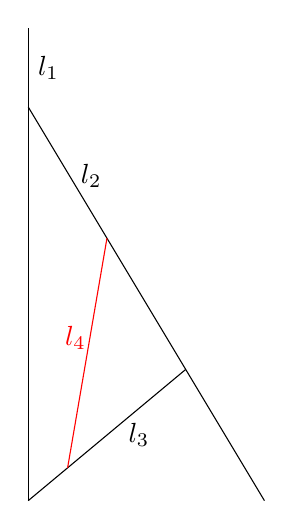
\begin{tikzpicture}
    % Draw a horizontal line
    \draw (0,0) -- (0,6);
    \node[right] at (0,5.5) {$l_{1}$};

    % Draw a line from (0,5) to (3,0) and label it
    \draw (0,5) -- (3,0);
    \node[below] at (0.8,4.4) {$l_{2}$};

    % Draw a line from (0,0) to (2.0, 5/3) and label it
    \draw (0,0) -- (2.0, 5/3);
    \node[right] at (1.15, 5/6) {$l_{3}$};

    % Draw a line from (1.0,10/3) to (0.5, 5/12) and label it
    \draw[red] (1.0,10/3) -- (0.5, 5/12);
    \node[above, text=red] at (0.6, 1.8) {$l_{4}$};
\end{tikzpicture}
\end{document}